\scanpage{80}
\mspage{39}
\[
\tag{\unsure{102|107}}
\diagram{\begin{tikzcd}[ampersand replacement=\&, column sep=large,row sep=large]
\& \Pi M^*_{\underline G,\underline G'} \arrow[r] \arrow[d] \& \Pi M_{G'} \\
\Pi(M_{\underline G}\deleted{,\unsure{\Gamma^!_{\underline G,\underline G'}}}) \arrow[r,"\approx"{name=equiv80}] \& \Pi M_{G,G'} \\
\& \begin{gathered}\text{ceci est une}\\\text{équivalence de}\\\text{groupoïdes}\end{gathered}
\arrow[from=equiv80,to=3-2,bend right=45]
\end{tikzcd}}
\]
qu'on va réécrire comme
\[
\tag{103}
\diagram{\begin{tikzcd}[ampersand replacement=\&, column sep=large,row sep=large]
\Pi M^*_{\underline G,\underline G'} \arrow[r,"\unsure{\gamma_{\underline G,\underline G'}|\psi_{\underline G,\underline G'}}"] \arrow[d,"\varphi_{G,G'}"] \& \Pi M_{G'} \\
\Pi(M_G,\deleted{\unsure{\Gamma^!_{\underline G,\underline G'}}})
\end{tikzcd}}
\]
\margin{``diagramme de générisation pour les groupoïdes fondamentaux pour le quotient de $\underline G\to\underline G'$''}
\deleted{\unsure{mais} pour la suite, il sera plus commode d'écrire $\Pi M_{G,G'}$ \unsure{au} lieu de $\Pi(M_G,\unsure{\Gamma^!_{\underline G,\underline G'}})$}

L'hom des groupoïdes $\varphi_{G,G'}$ propriétés de \deleted{\unsure{la}} l'hom sur les $\pi_1$ dans une fibration de base $(M_G\deleted{,\unsure{\Gamma_{\underline G,\underline G'}}\inserted{\text{op. de }\Gamma^!_{G,G'}}})$, \deleted{de} fibre un produit de disques épointés (ou de cercles, si on préfère) --- on peut considérer $\Pi M^*_{\underline G,\underline G'}$ comme une ``\uline{extension}'' canonique des groupoïdes $\Pi(M_G,\deleted{\unsure{\Gamma^!_{\underline G,\underline G'}}})$ par
\figure{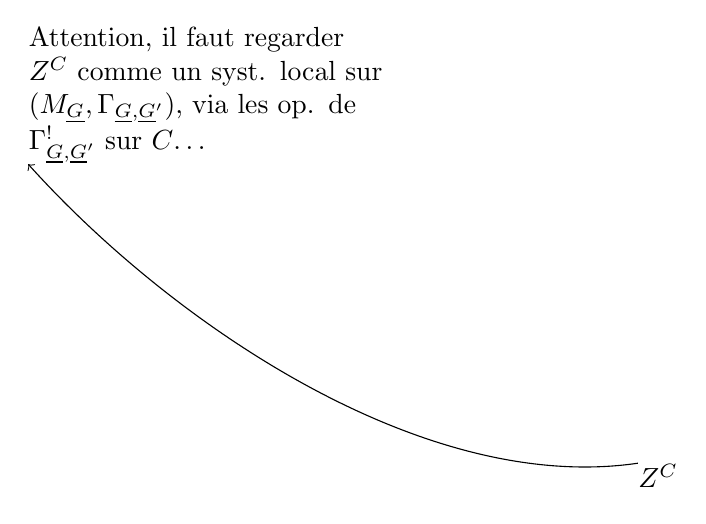
\begin{tikzpicture}[x=1cm,y=1cm]
\node[anchor=base,inner sep=0pt] (z80) at (8,0) {$\mathbb Z^C$};
\node[anchor=south west,align=left,text width=5cm,inner sep=0pt] (attention80) at (0,4.1) {Attention, il faut regarder $\mathbb Z^C$ comme un syst. local sur $(M_{\underline G},\Gamma_{\underline G,\underline G'})$, via les op. de $\Gamma^!_{\underline G,\underline G'}$ sur $C$\ldots};
\draw[->] (z80.north west) .. controls (5,-0.1) and (1.8,2.1) .. (attention80.south west);
\end{tikzpicture}}
, où $C$, on le rappelle, est l'ens. des \deleted{\unsure{flèches|frontières}}\inserted{arêtes} de $\underline G$
\margin{\uline{NB} $(M_G\deleted{,\unsure{\Gamma_{\underline G,\underline G'}}})$ est un $K(\pi,1)$, et par conséquent dans la suite exacte des $\pi_1$ de la fibration qui précède \unsure{incluse}, on a bien un $1$ à gauche}
\margin{79}
